
    \section{Coisas úteis}
    \subsection{Sequências}
        \begin{itemize}
            \item Primeiros números de Catalão: $1, 1, 2, 5, 14, 42, 132, 429, 1430, 4862, 16796, 58786, 208012, \\ 742900, 2674440, \dots$
            \item Primeiros números de Fibonnaci: $1, 1, 2, 3, 5, 8, 13, 21, 34, 55, 89, 144, 233, 377, 610, 987, 1597, 2584,  \\ 4181, 6765, 10946, \dots$
        \end{itemize}
        Os números de Fibonnaci também podem ser descritos como $f(n) = 4f(n-3) + f(n-6)$. Todos os $f(n)$ com $n = 2 ~(mod~3)$ tal que $f(0) = 1, f(1) = 1$ são pares.
    \subsection{Séries}
        \begin{minipage}{.48\textwidth}
        \subsubsection{PA}
            \begin{itemize}
                \item $a_n = a_{n-1} + r = a_0 + n \cdot r$
                \item $Soma(l,r) = \dfrac{(a_l + a_r) \cdot (r-l+1)}{2}$
            \end{itemize}
        \end{minipage}
        \begin{minipage}{.48\textwidth}
        \subsubsection{PG}
            \begin{itemize}
                \item $a_n = a_{n-1} \cdot  q = a_0 \cdot q^n$
                \item $Soma(l,r) = \dfrac{a_l \cdot  (q^{r-l+1} - 1)}{q-1}$
            \end{itemize}
        \end{minipage}
    \subsection{Identidades Binomiais}
    $$
        \begin{array}{cc}
        \binom{n}{k} = \binom{n}{n-k} & 
        \binom{n}{k} = \frac{n}{k}\binom{n-1}{k-1} 
        \\[10pt]
        \sum_{k = 0}^n \binom{n}{k} = 2^n & 
        \binom{n}{0} + \binom{n}{2} + \binom{n}{4} + \dots + \binom{n}{\lfloor \frac{n}{2} \rfloor \cdot 2} = 2^{n-1}
        \\[10pt]
        \sum_{k = 0}^m \binom{n+k}{k} = \binom{n+m+1}{m} & 
         \sum_{m = k}^n \binom{m}{k} = \binom{n+1}{k+1}
        \\[10pt]
        \sum_{k = 0}^n k\binom{n}{k} = n 2^{n-1} &
        2\sum_{i = L}^R \binom{n}{i} - \binom{n}{L} - \binom{n}{R} = \sum_{i = L+1}^R \binom{n+1}{i}
        \\[10pt]
        \binom{n}{h}\binom{n-h}{k} = \binom{n}{k}\binom{n-k}{h} &
        \binom{n}{k} = \frac{n+1-k}{k} \binom{n}{k-1}
        \\[10pt]
         \binom{n-1}{k} - \binom{n-1}{k-1} = \frac{n - 2k}{k} \binom{n}{k} &
        \sum_{k = 0}^n k^2 \binom{n}{k} = (n + n^2)2^{n-2}
        \\[10pt]
        \sum_{j = 0}^k\binom{m}{j} \binom{n-m}{k-j} = \binom{n}{k} &
        \sum_{j = 0}^m \binom{m}{j}^2 = \binom{2m}{m}
        \\[10pt]
        \sum_{m = 0}^n \binom{m}{j} \binom{n-m}{k-j} = \binom{n+1}{k+1} & 
        \sum_{k=0}^{\lfloor n/2 \rfloor} \binom{n-k}{k} = \text{Fib}(n+1)
        \\[10pt] 
        (x + y)^{n} = \sum_{k=0}^{n} \binom{n}{k} x^{n-k} y^{k} &
        (1 + x)^{n} = \sum_{k=0}^{n} \binom{n}{k} x^{k}
        \\[10pt]
        \end{array}
    $$
    \subsection{Geometria}
        \subsubsection{Triângulos}
            Qualquer triângulo retângulo ($a^2 + b^2 = c^2$) com lados coprimos pode ser gerado escolhendo um par de inteiros coprimos $m > n > 0$ em que exatamente um deles é par. Com lados iguais: $a = m^2 - n^2$, $b = 2mn$ e $c = m^2 + n^2$. Isso vem de $a^2 + b^2 = c^2$
            \begin{center}
                \begin{minipage}{.48\textwidth}
                \centering
                    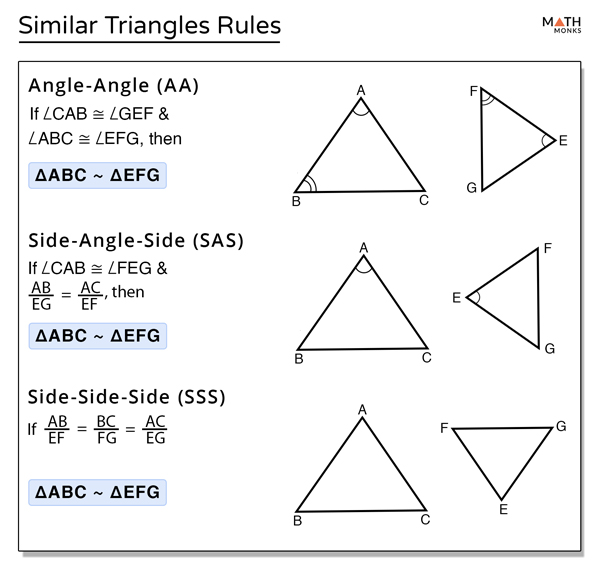
\includegraphics[scale=0.3]{imgs/Similar-Triangles-Rules.jpg}
                    \captionof{figure}{Similaridade de triângulos}
                \end{minipage}
                \begin{minipage}{.48\textwidth}
                \centering
                    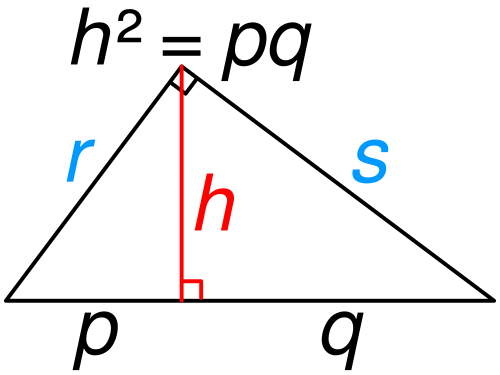
\includegraphics[scale=0.3]{imgs/Right_angle_altitude.png}
                    \captionof{figure}{Altura de triângulo retângulo}
                \end{minipage}
            \end{center}
            
            \paragraph{Trigonometria}
                \begin{center}
                    \begin{minipage}{.48\textwidth}
                        \centering
                        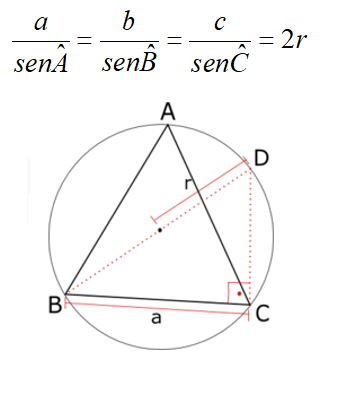
\includegraphics[scale=0.4]{imgs/leidossenos.png}
                        \captionof{figure}{Lei dos senos}
                    \end{minipage}
                    \begin{minipage}{.48\textwidth}
                    \centering
                        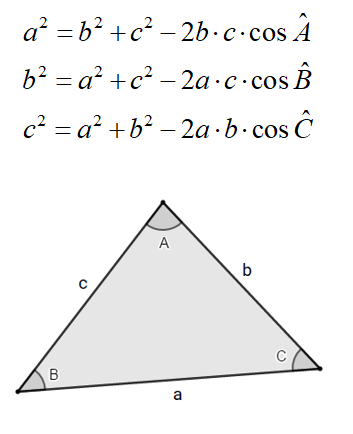
\includegraphics[scale=0.4]{imgs/leidoscosenos.png}
                        \captionof{figure}{Lei dos cossenos}
                    \end{minipage}
                    \begin{minipage}{.48\textwidth}
                    \centering
                        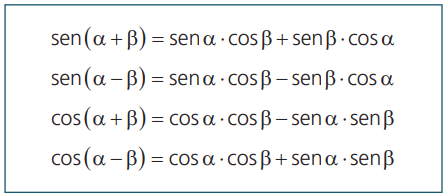
\includegraphics[scale=0.4]{imgs/soma_arcos.png}
                        \captionof{figure}{Soma de arcos}
                    \end{minipage}
                \end{center}
            
        \subsubsection{Fórmula de Heron}
        Calcular área de polígonos usando a medida dos lados, considere $a_i$ o $i$-ésimo lado e $p = \displaystyle \frac{\sum_{i=0}^n a_i}{2}$ o semiperímetro de um polígono.
            \begin{itemize}
                \item Triângulo: $A = \sqrt{p \cdot (p-a_0) \cdot (p-a_1) \cdot (p-a_2)}$
                \item Quadrilátero inscritível: $A = \sqrt{(p-a_0) \cdot (p-a_1) \cdot (p-a_2) \cdot (p-a_3)}$
                \item Quadrilátero qualquer: $A = \sqrt{(p-a_0) \cdot (p-a_1) \cdot (p-a_2) \cdot (p-a_3)  - a_0a_1a_2a_3 \cdot \cos(\frac{\alpha + \gamma}{2})}$, onde $\alpha,\gamma$ são ângulos opostos quaisquer
            \end{itemize}
    \subsection{Cálculo}
        \subsubsection{Multiplicadores de Lagrange}
        Dado uma função $f(x_1,x_2,\dots, x_n)$ com restrições $g_i(x_1,x_2,\dots,x_n) = k_i$ onde $1 \le i \le m$ e $m$ é o número de restrições, queremos otimizá-la. Usando o método dos multiplicadores de Lagrange, conseguimos reduzir o problema a resolver o sistema de equações:
        \[
            \left\{
            \begin{array}{{rcl}}
               \nabla f(x_1,x_2,\dots,x_n) & = & \sum_{i=1}^{m} \lambda_i \nabla g_i(x_1,x_2,\dots,x_n)  \\
                g_i(x_1,x_2,\dots,x_n)     & = & k_i \ \ \ \ \ \ \ \text{for $1 \le i \le m$}
            \end{array}
            \right.
        \]
        
        Para a primeira equação, você deriva a função para cada variável e resolve pra cada derivada parcial (vai ser um vetor de equações).

    \subsection{Polinômio}
        Se você acha que alguma função vira um polinômio de grau $k$, calcula o valor dessa função para $k+1$ valores e descobre os coeficientes do polinômio por um sistema linear. Exemplo $f(n) = \sum_{i=1}^n i$ pode ser um polinômio da forma $p(x) = ax^3 + bx^2 + cx + d$, calcula o valor de $f(n)$ para $0,1,2,3$ e calcula os coeficientes.
    \subsection{Teoria dos números}
        \subsubsection{Teorema de Fermat-Lagrange}
        \begin{minipage}{.48\textwidth}
        Todo inteiro pode ser escrito como:
        \begin{itemize}
            \item soma de no máximo 3 números triangulares,
            \item soma de no máximo 4 números quadrados,
            \item soma de no máximo 5 números pentagonais,
            \item \dots
        \end{itemize}
        O $i$-ésimo número $n$-gonal é a quantidade de pontos na construção do $i$-ésimo $n$-polígono conforme a figura. Sempre vai ter uma fórmula fechada para calcular esses números.
        \end{minipage}
        \begin{minipage}{.48\textwidth}
        \centering
        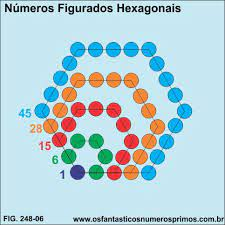
\includegraphics[scale=0.7]{imgs/ngonal.jpeg}
        \end{minipage}

        \subsubsection{Números primos}

        Todo $n \neq 2,3$ primo é da forma $6k \pm 1$. Pois qualquer outra forma de $6k + r$ com $0 \leq r < 5$ não é primo. Então você pode testar primo andando só de 6 em 6.
    \subsection{Probabilidade}
        \subsubsection{Valor esperado}
            Se $E(x) = \sum_{i=1}^x i\cdot P(x=i)$ com $P(x = i)$ sendo a probabilidade da variável $x$ ser igual a $i$, podemos reescrever como $E(x) = \sum_{i=1}^xP(x\geq i)$.
    \newpage
